\documentclass[]{article}
\usepackage{amssymb,amsmath}
\usepackage{ifxetex,ifluatex}
\ifxetex
  \usepackage{fontspec,xltxtra,xunicode}
  \defaultfontfeatures{Mapping=tex-text,Scale=MatchLowercase}
  \newcommand{\euro}{€}
\else
  \ifluatex
    \usepackage{fontspec}
    \defaultfontfeatures{Mapping=tex-text,Scale=MatchLowercase}
    \newcommand{\euro}{€}
  \else
    \usepackage[utf8]{inputenc}
    \usepackage{eurosym}
  \fi
\fi
% Redefine labelwidth for lists; otherwise, the enumerate package will cause
% markers to extend beyond the left margin.
\makeatletter\AtBeginDocument{%
  \renewcommand{\@listi}
    {\setlength{\labelwidth}{4em}}
}\makeatother
\usepackage{enumerate}
\usepackage{graphicx}
% We will generate all images so they have a width \maxwidth. This means
% that they will get their normal width if they fit onto the page, but
% are scaled down if they would overflow the margins.
\makeatletter
\def\maxwidth{\ifdim\Gin@nat@width>\linewidth\linewidth
\else\Gin@nat@width\fi}
\makeatother
\let\Oldincludegraphics\includegraphics
\renewcommand{\includegraphics}[1]{\Oldincludegraphics[width=\maxwidth]{#1}}
\ifxetex
  \usepackage[setpagesize=false, % page size defined by xetex
              unicode=false, % unicode breaks when used with xetex
              xetex,
              colorlinks=true,
              linkcolor=blue]{hyperref}
\else
  \usepackage[unicode=true,
              colorlinks=true,
              linkcolor=blue]{hyperref}
\fi
\hypersetup{breaklinks=true, pdfborder={0 0 0}}
\setlength{\parindent}{0pt}
\setlength{\parskip}{6pt plus 2pt minus 1pt}
\setlength{\emergencystretch}{3em}  % prevent overfull lines
\setcounter{secnumdepth}{0}


\begin{document}

\section{What does a
\href{http://en.wikipedia.org/wiki/Revision\_control}{Version Control
System} do?}

\begin{itemize}
\item
  Track source code
  \begin{itemize}
  \item
    Maintain code history, integrity, atomic change\ldots{}
  \end{itemize}
\item
  Coordinate distributed development
  \begin{itemize}
  \item
    branch, merge conflicts, tag\ldots{}
  \end{itemize}
\end{itemize}
\begin{figure}[htbp]
\centering
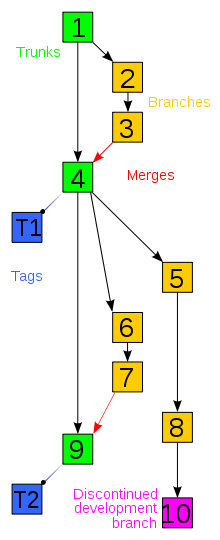
\includegraphics{figures/vcsflow.png}
\caption{VCS general work flow}
\end{figure}

\section{VCS Work Flow Categories}

\begin{itemize}
\item
  Centralized:
  \href{http://msdn.microsoft.com/en-us/library/3h0544kx(v=vs.80).aspx}{VSS},
  \href{http://www.nongnu.org/cvs/}{CVS},
  \href{http://subversion.apache.org/}{SVN}
\item
  Distributed{[}\^{}dvcsflow{]}
  \href{http://www.bitkeeper.com/}{BitKeeper},
  \href{http://git-scm.com/}{git},
  \href{http://mercurial.selenic.com/\%20{[}\^{}dvcsflow{]}:\%20Distributed\%20VCSs\%20support\%20centralized\%20work\%20flow\%20too.}{mercurial}\ldots{}
\end{itemize}
\section{Why git is better than X (SVN, CVS, \ldots{})}

\begin{itemize}
\item
  git is super fast
\item
  Full repository clone
\item
  Local history: no need to connect to servers when viewing the revision
  history
\item
  Cheap branch and easy merge
\item
  {[}github{]}: social coding\footnote{\href{https://bitbucket.org}{bitbucket},
    \href{http://code.google.com}{Google Code} support git too, but
    github in no doubt has more
    \href{http://shop.github.com/}{\emph{fun}}.}
\item
  Other things: tidy working directory, better compression, multi work
  flow support, \ldots{}
\end{itemize}
\section{General Advice on Learning git}

\begin{itemize}
\item
  Try git and {[}github{]}
\item
  Most graphical tool/plug-ins\footnote{\href{http://code.google.com/p/tortoisegit/}{tortoisegit},
    \href{http://lostechies.com/joshuaflanagan/2010/09/03/use-gitk-to-understand-git/}{gitk},
    \href{http://www.eclipse.org/egit/}{EGit},
    \href{https://github.com/blog/1067-github-for-mac-1-2-snow-octocat}{Snow
    Octocat}\ldots{} But please, oh please use the command-line tool.
    {[}github{]}: https://github.com/} \emph{SUCK}. Please use the
  command-line git.
\item
  Read git's prompts, run \textbf{git help} to get help.
\item
  Find ``how-to'' on Google, StackOverflow, git book.
\end{itemize}
\section{Rules of Thumb for git}

\begin{itemize}
\item
  ``A clear development flow is worth thousands of VCSs.''
\item
  Modular design, avoid simultaneous source file editing by different
  members.
\item
  Head version at trunk is always ready to deploy.
\item
  Modification is made on branches, then merged into trunk.
\item
  Stay on your own branch.
\item
  Write comment to each commit.
\end{itemize}
\section{To get started, I will\ldots{}}

\begin{itemize}
\item
  Illustrate git's various work flows.
\item
  Explain the most frequently used git commands.
\item
  Give exercises for self check. Some of the exercises require github
  access.
\end{itemize}
\section{git's stand-alone work flow}

\begin{itemize}
\item
  You can use git on a stand-alone computer and easily integrate the
  code into a more sophisticated work flow (distributed or centralized)
  at a later time.
\end{itemize}
\begin{figure}[htbp]
\centering
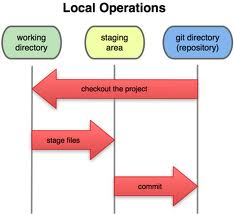
\includegraphics{figures/gitstandalone.jpeg}
\caption{gitalone}
\end{figure}

\section{git's distributed work flow}

\begin{itemize}
\item
  Every collaborator keeps a full clone of the repository.
\item
  All repositories are peers.
\item
  Repositories are not necessarily consistent at all time. Use push/pull
  to exchange changes when neccessary.
\end{itemize}
\begin{figure}[htbp]
\centering
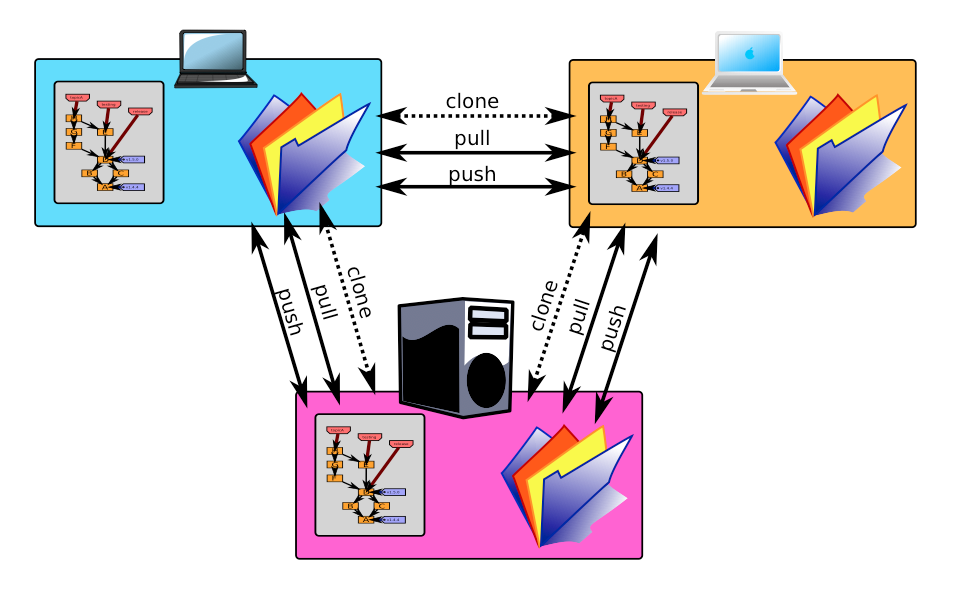
\includegraphics{figures/gitdvcs.png}
\caption{gitdvcs}
\end{figure}

\section{git's emulation to the centralized work flow
(\textbf{RECOMMENDED})}

\begin{itemize}
\item
  It's \textbf{emulation}, not \emph{real}.\\
\item
  The statement, ``all repositories are peers.'', still holds.
\item
  We pretend that we see the central repo only, unaware of each other's
  peer repo.
\end{itemize}
\begin{figure}[htbp]
\centering
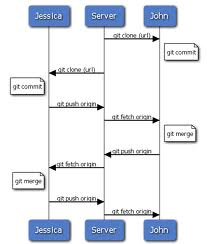
\includegraphics{figures/gitcent.jpeg}
\caption{gitcent}
\end{figure}

\section{Set up git}

\begin{itemize}
\item
  Please follow github's nice tutorials to set up\footnote{The email you
    fill in when signing up is used for web login and password reset
    only. github uses SSH keys for \emph{git} authentication. Try to
    clarify the following \emph{pass phrases}: your email account's pass
    phrase, your github account's pass phrase, and the pass phrase to
    access your SSH private key. {[}gitonwin{]}:
    http://help.github.com/win-set-up-git/ {[}gitonlinux{]}:
    http://help.github.com/linux-set-up-git {[}gitonmac{]}:
    http://help.github.com/mac-set-up-git/} git on
  {[}Windows{]}{[}gitonwin{]}, {[}Linux{]}{[}gitonlinux{]} or
  {[}Mac{]}{[}gitonmac{]}.
\item
  {[}Must-known things about SSH keys{]}{[}sshthings{]}: private key,
  public key, the pass phrase to access the private key, key
  fingerprint.
\item
  Don't forget to set \emph{user.name} and \emph{user.email}\footnote{Usernames
    and emails in git's configuration are for identification purpose
    only, not for sending emails. It is highly recommended that the
    email in git and SSH keeps the same. {[}sshthings{]}:
    http://linux.vbird.org/linux\_server/0310telnetssh.php\#ssh\_server}
  before your very first git commit.
\end{itemize}
\section{git command}

\begin{itemize}
\item
  help
\item
  init
\item
  status
\item
  add
\item
  commit
\item
  diff
\item
  tag
\item
  Working with branch
\item
  Working with remotes
\item
  submodule
\item
  Oh, there is a conflict!!!
\item
  ``Time Machine'': stash, stash list, checkout to a commit, checkout to
  master
\end{itemize}
\section{\emph{help}: Get help}

\emph{git help COMMAND} Get help from git. + \emph{git help add} +
\emph{git help commit} + \ldots{}

\section{\emph{init}: Initialize a local git repo for your project}

\emph{init} command will create a \emph{.git} dir on the top level of
your project.\\ + \emph{cd YOUR\_REPO\_DIR} + \emph{git init .}

\section{\emph{status}: Show the status of your repo}

\emph{git status} + \emph{status} tells you how to \textbf{UNDO} the
last operation on git +
\href{http://progit.org/book/ch2-2.html\%20{[}\^{}commitstatus{]}:\%20The\%20*committed*\%20status\%20simply\%20displays\%20nothing\%20when\%20running\%20*git\%20status*.}{File
status}: \emph{untracked}, \emph{unstaged}, \emph{staged} (indexed),
\emph{committed}{[}\^{}commitstatus{]}

\begin{figure}[htbp]
\centering
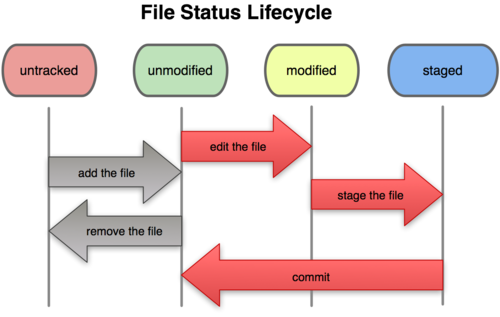
\includegraphics{figures/gitlifecycle.png}
\caption{gitlifecyle}
\end{figure}

\section{\emph{add}: A multi-function git command}

\emph{git add FILES\_OR\_DIR}\\ + For untracked files: \emph{add} them
to git's control + For unstaged changes: \emph{add} them to the staged
area + For conflicted files: \emph{add} marks them as ``resolved''

\section{commit: Store the status (snapshot) permanently}

\begin{itemize}
\item
  \emph{git commit -m ``YOUR\_COMMENT''}
\item
  \emph{git commit} stores the STAGED changes only
\item
  \emph{git commit -a} stores all the STAGED and UNSTAGED changes.
\item
  Each commit is identified by a \textbf{UNIQUE} SHA-1 ID of 40 ASCII
  characters.
\item
  Please write comment for each of your commit.

  commit dd5f924c40096b9cda27ffd1cfd1205822ab3c70 Author: Jianwen Wei
  \href{mailto:wei.jianwen@gmail.com}{\texttt{wei.jianwen@gmail.com}}
  Date: Sun Apr 1 19:38:37 2012 +0800

\begin{verbatim}
Restart the git-tutorial project.
\end{verbatim}
\end{itemize}
\section{diff: Find differences}

\begin{itemize}
\item
  \emph{git diff}
\item
  changes between the staged and working files
\item
  \emph{git diff --staged}
\item
  changes between the HEAD and the staged files
\item
  \emph{git diff HEAD}
\item
  changes between the HEAD and the working files
\item
  \emph{git diff COMMIT\_ID COMMIT\_ID}
\item
  changes between two commits
\end{itemize}
\section{tag: A milestone version}

\begin{itemize}
\item
  \emph{git tag}
\item
  See all the tag
\item
  \emph{git show TAG\_NAME}
\item
  See a tag in detail
\item
  \emph{git TAG\_NAME}
\item
  Add a ``lightweight'' tag
\item
  \emph{git -a TAG\_NAME -M YOUR\_COMMENT}
\item
  Add a tag
\item
  \emph{git tag -d TAG\_NAME}
\item
  Delete a tag
\end{itemize}
\section{Submodule: Integrate multi git repos}

\begin{itemize}
\item
  \emph{git help submodule}
\item
  \href{http://progit.org/book/ch6-6.html}{Repo in Repo}
\item
  Manage other repos as ``submodules'' in your project
\end{itemize}
\section{Working with \textbf{branch}: branch, checkout, merge}

A branch-based development flow: 1. Create a branch 2. Switch to the
newly-created branch 3. Modify and commit on the branch 4. Merge
branch's changes into trunk.

\section{Working with \textbf{branch}: \emph{branch}, checkout, merge}

\begin{itemize}
\item
  \emph{git branch} See all the branches
\item
  \emph{git branch BRANCH\_NAME} Create a branch
\item
  \emph{git branch -d BRANCH\_NAME} Delete a branch
\item
  \emph{git branch -D BRANCH\_NAME} Force delete a branch
\end{itemize}
\section{Working with \textbf{branch}: branch, \emph{checkout}, merge}

\begin{itemize}
\item
  \emph{git checkout BRANCH\_NAME} Switch to a branch. The working files
  will change.\footnote{Don't confuse git's term \emph{checkout} here
    with subversion's checkout.}
\item
  \emph{git checkout -f BRANCH\_NAME} Force switch to a branch
\item
  \emph{git checkout master} Go back to trunk, named \emph{master} in
  git.
\item
  \emph{git checkout -b BRANCH\_NAME} Create a branch then switch to it.
\end{itemize}
\section{Working with \textbf{branch}: branch, checkout, \emph{merge}}

\begin{itemize}
\item
  \emph{git merge BRANCH\_A BRANCH\_B} Merge branch\_a's and branch\_b's
  changes into \emph{current} branch
\item
  \emph{git checkout master, git merge master BRANCH\_NAME} Merge
  changes into trunk--the master branch.
\end{itemize}
\section{Working with \textbf{remotes}: \emph{clone}, remote, push,
pull}

\begin{itemize}
\item
  \emph{git clone REPO\_URL} Full clone of a repo.
\item
  URL can be in forms of local dir (\textasciitilde{}/proj), git
  (git://xxx), SSH (ssh://xxx), https (http://xxx)\ldots{}
\end{itemize}
\section{Working with \textbf{remotes}: clone, \emph{remote}, push,
pull}

\begin{itemize}
\item
  \emph{remote} manages the set of tracked repositories.\footnote{Remote
    repos in git are just references or pointers, so you lose or gain
    \emph{nothing} when adding or removing a remote repo.}
\item
  \emph{git remote} Show all the tracked repositories.
\item
  \emph{git remote show REPO\_NAME} Show the repo's details.
\item
  \emph{git remote add REPO\_NAME REPO\_URL} Add a remote repo to
  tracked list.
\item
  \emph{git remote -d REPO\_NAME} Remove a remote repo from the tracked
  list. \# \emph{git remote rename REPO\_OLD REPO\_NEW} Rename a repo.
\end{itemize}
\section{Working with \textbf{remotes}: clone, remote, \emph{push,
pull}}

\begin{itemize}
\item
  \emph{git pull REPO\_NAME BRANCH\_NAME} Merge remote branch's changes
  into current branch.
\item
  \emph{git push REPO\_NAME BRANCH\_NAME} Push current branch's changes
  to the remote branch.
\end{itemize}
\section{Oh, there is a conflict!!!}

\begin{itemize}
\item
  A conflict looks like:
  \texttt{\textless{}\textless{}\textless{}\textless{}\textless{}\textless{}\textless{} HEAD:index.html \textless{}div id="footer"\textgreater{}contact : email.support@github.com\textless{}/div\textgreater{} ======= \textless{}div id="footer"\textgreater{}   please contact us at support@github.com \textless{}/div\textgreater{} \textgreater{}\textgreater{}\textgreater{}\textgreater{}\textgreater{}\textgreater{}\textgreater{} iss53:index.html}
\item
  Conflicts arise when git cannot automatically merge changes at
  \emph{merge} or \emph{pull} operations.
\item
  Don't panic. Conflicts are no big deal, sometimes even inevitable.
\item
  What you should do: merge the conflicts, mark the files as
  ``resolved'', then commit the changes.
\end{itemize}
\section{Working with conflicts: merge, resolve, commit}

\begin{enumerate}[1.]
\item
  You have to edit the conflicted files, merge conflicts MANUALLY.
  \emph{diff} command may help you.
\item
  \emph{git add CONFLICT\_FILES} Mark the file as resolved.
\item
  \emph{git commit -m ``YOUR\_COMM''} Commit changes to the repo.
\end{enumerate}
\section{``Time Machine'': \emph{stash}, checkout}

\emph{stash} saves your temporary work and resets the files to HEAD
version. You can handle some emergency fix first then continue to hack
at a latter time.

\begin{enumerate}[1.]
\item
  \emph{git stash} Save the temp changes.
\item
  \emph{git stash list} Check the stash list.
\item
  EDIT and COMMIT your emergency fix.
\item
  \emph{git stash pop} Continue to hack
\end{enumerate}
\section{``Time Machine'': stash, \emph{checkout}}

\emph{checkout} enable you to go backward and forward in the revision
history. 1. \emph{git checkout COMMITID\_OR\_TAGNAME} \footnote{The full
  commit ID is 40 characters long. But you may type a short prefix (like
  4\textasciitilde{}6 characters) to refer a commit uniquely.} 2. You
are on a \emph{unnamed} branch with file status dating back. Do anything
you want. 3. \emph{git checkout master} Come back to master.

\section{Exercise: git environment}

\section{Exercise: diff}

\section{Exercise: branch}

\section{Exercise: github}

\section{Exercise: Remote Branch}

\section{Exercise: Conflicts}

\section{Exercise: tag}

\section{Exercise: Time Machine}

\end{document}
